% Figura Anexo II: sustitución intertemporal del trabajo: una subida transitoria del salario mueve las horas; una permanente, no
\documentclass[tikz,border=3pt]{standalone}
\usepackage[T1]{fontenc}
\usepackage[utf8]{inputenc}
\usepackage{amsmath}
\usetikzlibrary{arrows.meta,calc,positioning}
\begin{document}
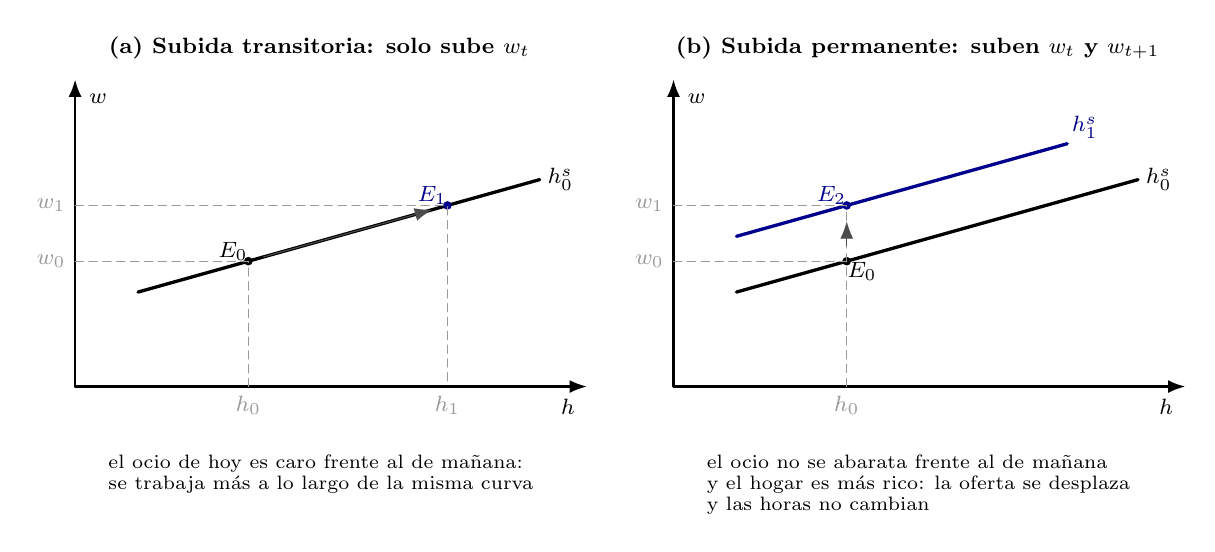
\begin{tikzpicture}[>={Latex[length=2.2mm]}, line cap=round, font=\footnotesize,
  eje/.style={->, thick},
  curva/.style={very thick},
  nueva/.style={very thick, blue!55!black},
  guia/.style={densely dashed, gray!80},
  pto/.style={circle, fill=black, inner sep=1.1pt}]
  % ---------- Panel (a): subida transitoria ----------
  \node[font=\footnotesize\bfseries] at (3.1,4.3) {(a) Subida transitoria: solo sube $w_t$};
  \draw[eje] (0,0) -- (6.5,0) node[below left=1pt]{$h$};
  \draw[eje] (0,0) -- (0,3.9) node[below right=2pt]{$w$};
  \draw[curva] (0.8,1.2) -- (5.9,2.628) node[right=-1pt]{$h^{s}_{0}$};
  \node[pto] (E0) at (2.2,1.592) {};
  \node[above left=-3pt of E0, inner sep=1pt] {$E_0$};
  \node[pto, fill=blue!55!black] (E1) at (4.729,2.3) {};
  \node[above left=-3pt of E1, inner sep=1pt, blue!55!black] {$E_1$};
  \draw[guia] (0,1.592) node[left]{$w_0$} -- (2.2,1.592) -- (2.2,0) node[below]{$h_0$};
  \draw[guia] (0,2.3) node[left]{$w_1$} -- (4.729,2.3) -- (4.729,0) node[below]{$h_1$};
  \draw[->, gray!60!black, shorten >=4pt, shorten <=4pt] (E0) -- (E1);
  \node[align=left, anchor=north west] at (0.3,-0.75) {\scriptsize el ocio de hoy es caro frente al de mañana:\\[-2pt]\scriptsize se trabaja más a lo largo de la misma curva};
  % ---------- Panel (b): subida permanente ----------
  \begin{scope}[xshift=7.6cm]
    \node[font=\footnotesize\bfseries] at (3.1,4.3) {(b) Subida permanente: suben $w_t$ y $w_{t+1}$};
    \draw[eje] (0,0) -- (6.5,0) node[below left=1pt]{$h$};
    \draw[eje] (0,0) -- (0,3.9) node[below right=2pt]{$w$};
    \draw[curva] (0.8,1.2) -- (5.9,2.628) node[right=-1pt]{$h^{s}_{0}$};
    \draw[nueva] (0.8,1.908) -- (5.0,3.084) node[above right=-3pt]{$h^{s}_{1}$};
    \node[pto] (F0) at (2.2,1.592) {};
    \node[below right=-3pt of F0, inner sep=1pt] {$E_0$};
    \node[pto, fill=blue!55!black] (F2) at (2.2,2.3) {};
    \node[above left=-3pt of F2, inner sep=1pt, blue!55!black] {$E_2$};
    \draw[guia] (0,1.592) node[left]{$w_0$} -- (2.2,1.592);
    \draw[guia] (0,2.3) node[left]{$w_1$} -- (2.2,2.3) -- (2.2,0) node[below]{$h_0$};
    \draw[->, gray!60!black, shorten >=4pt, shorten <=4pt] (F0) -- (F2);
    \node[align=left, anchor=north west] at (0.3,-0.75) {\scriptsize el ocio no se abarata frente al de mañana\\[-2pt]\scriptsize y el hogar es más rico: la oferta se desplaza\\[-2pt]\scriptsize y las horas no cambian};
  \end{scope}
\end{tikzpicture}
\end{document}
